% References:
%   [1] https://tex.stackexchange.com/questions/118069/how-to-draw-an-euler-angle-rotation-sequence-with-tikz
%   [2] https://tex.stackexchange.com/questions/218354/i-want-to-draw-a-dot-small-sphere-in-a-tikz-3d-plot

% ---------
% Preamble.
% ---------

% Document type.
\documentclass{article}

% Import custom style.
\usepackage{../.preamble/tikz_diagrams_template}

% Color theme (black, red, blue, green, orange, purple, gold).
\colortheme{blue}

% ---------
% Document.
% ---------

\begin{document}

    % Sets viewing orientation (declination/rotation) of 3D coordinate system.
    \tdplotsetmaincoords{90}{0}
    % \tdplotsetmaincoords{60}{140}

    % Change rotation matrix to use 3-2-1 sequence.
    \tdseteulerxyz

    % -----------------
    % TikZ environment.
    % -----------------

    \begin{tikzpicture}[tdplot_main_coords,scale=1]
        
        % Rocket drawing.
        \node[anchor=south west,inner sep=0] (image) at (0,0) {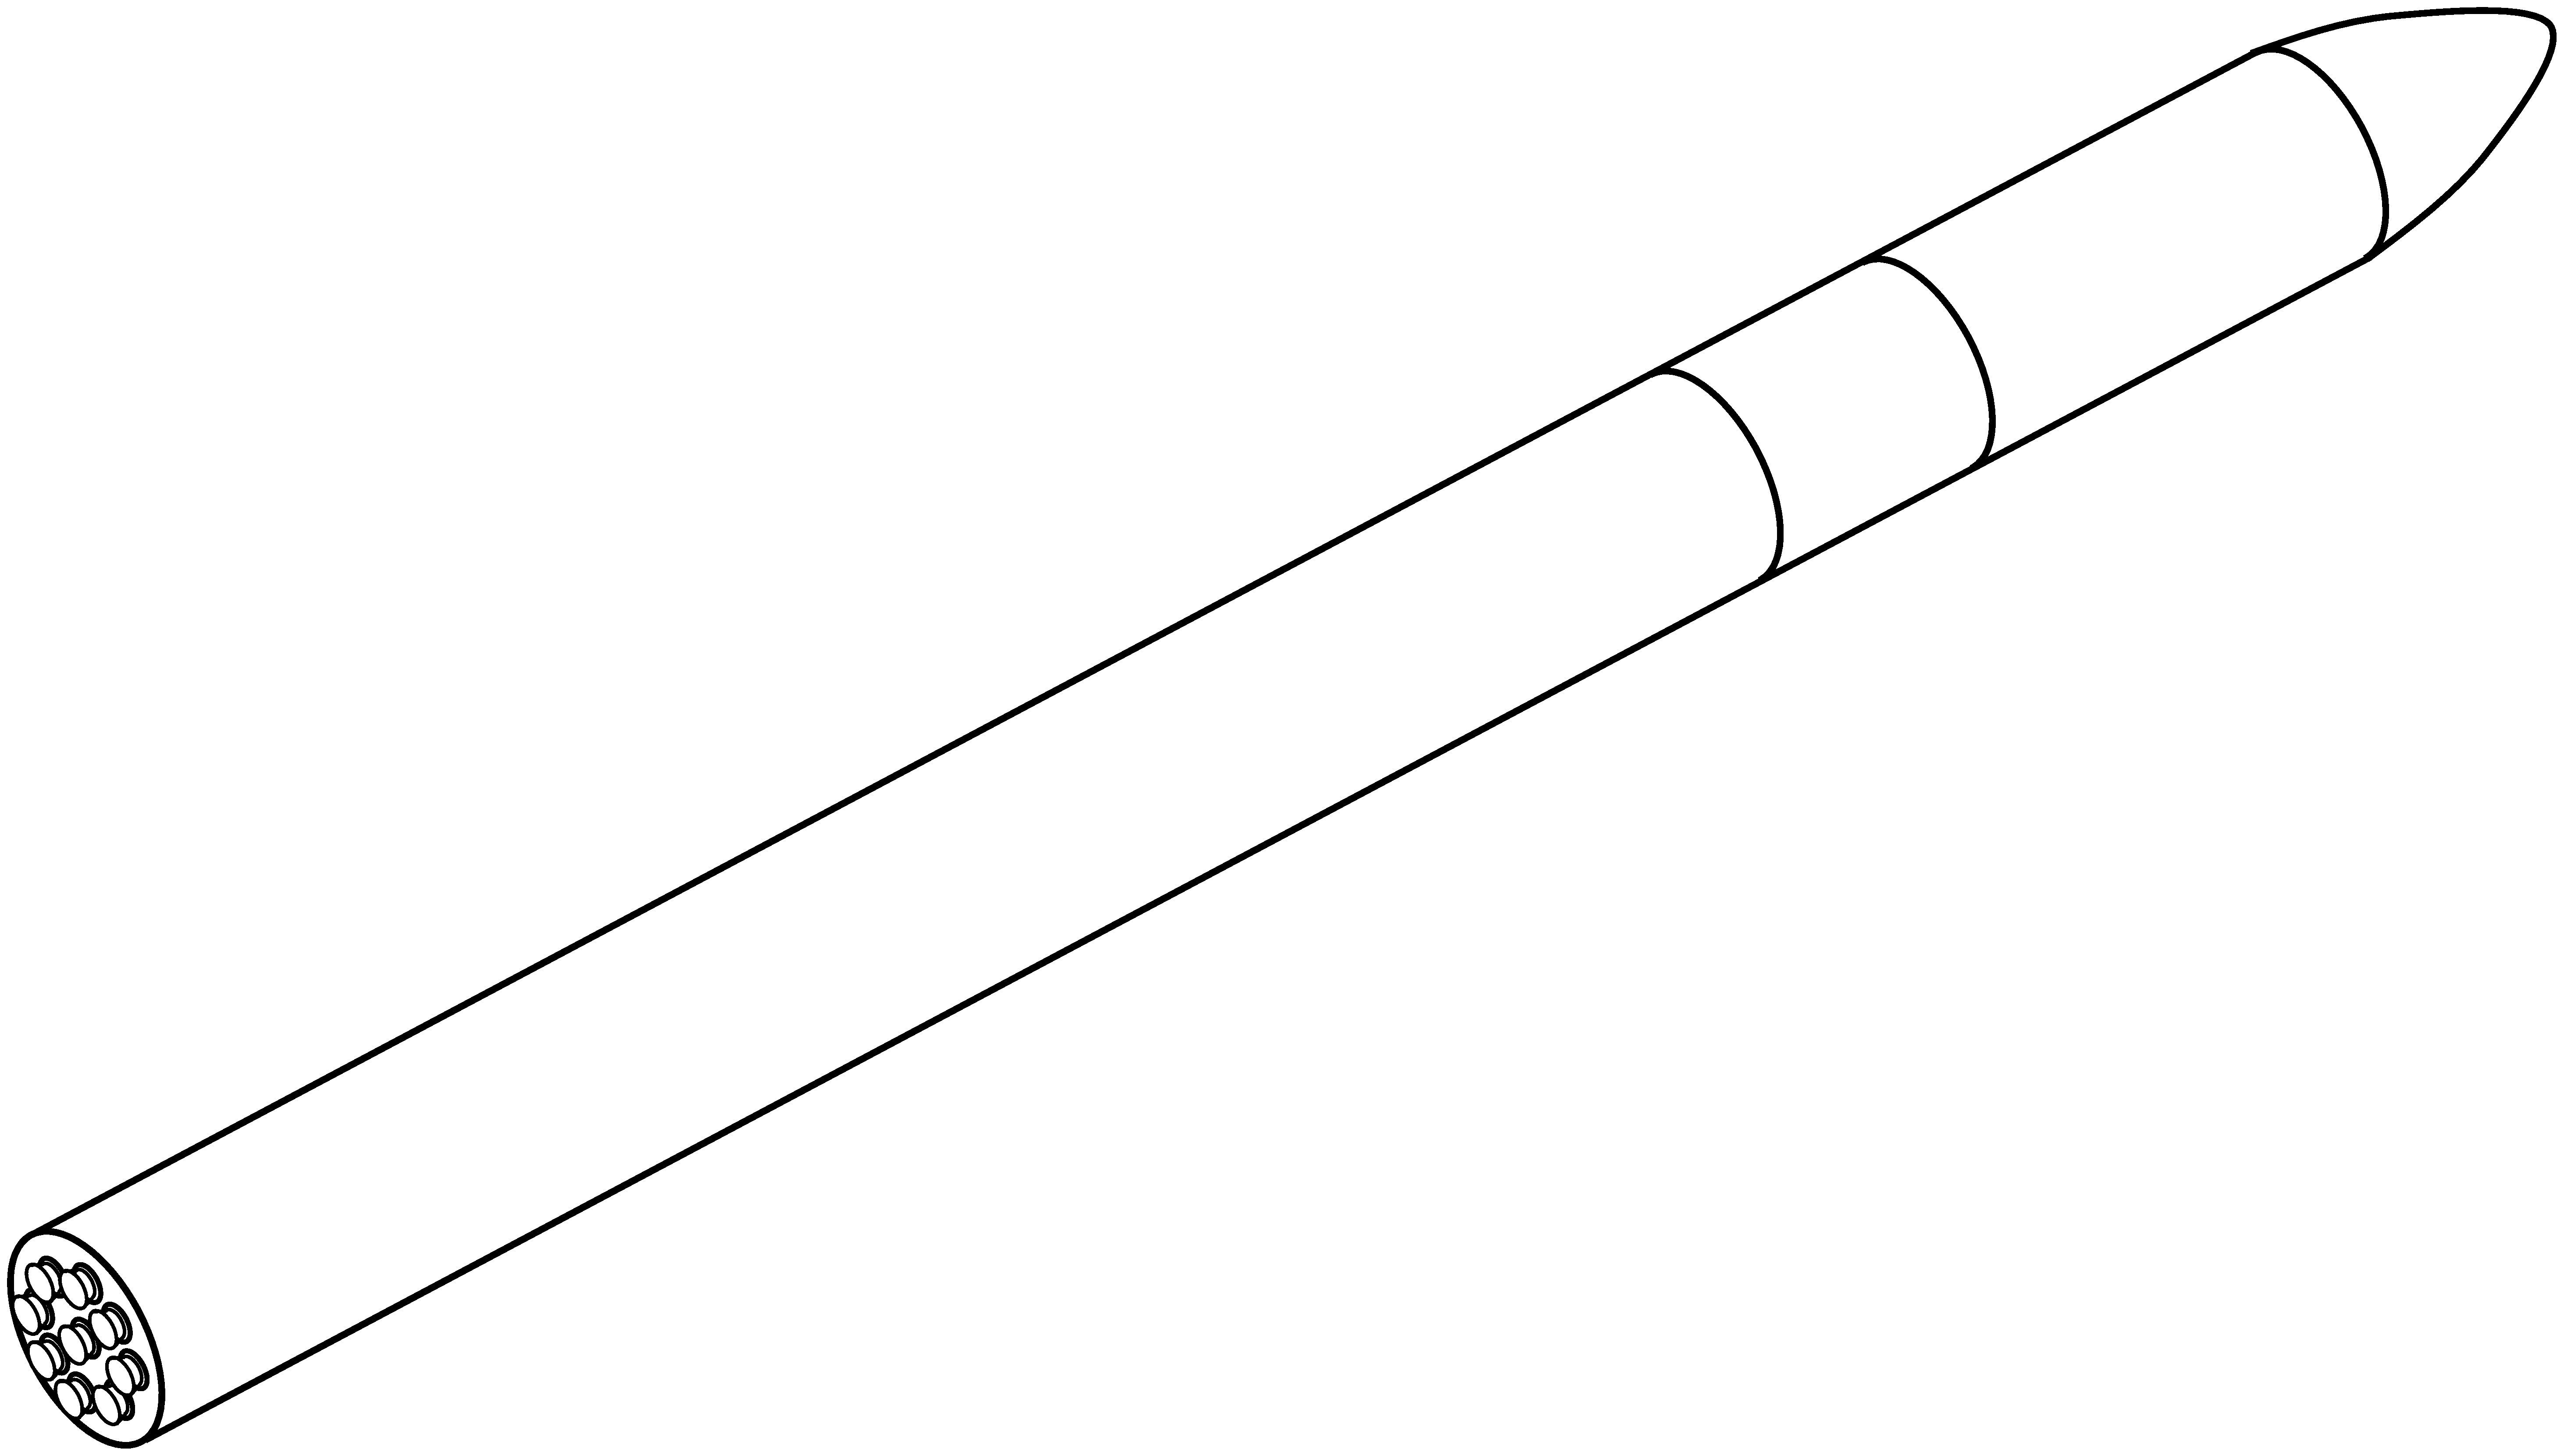
\includegraphics[width=0.3\textwidth]{../.images/rocket.eps}};
        
        % Axes length.
        \pgfmathsetmacro{\axlen}{3}
    
        % Scope to draw world axes.
        \begin{scope}[x={(image.south east)},y={(image.north west)}]
            
            % Rotation angles to align with world frame [deg].
            \pgfmathsetmacro{\zRotw}{230}
            \pgfmathsetmacro{\yRotw}{20}
            \pgfmathsetmacro{\xRotw}{-15}

            % Rotates TikZ's coordinate system to align with world frame.
            \tdplotsetrotatedcoords{\zRotw}{\yRotw}{\xRotw}

            % World origin.
            \pgfmathsetmacro{\Oxw}{3}
            \pgfmathsetmacro{\Oyw}{-3}
            \pgfmathsetmacro{\Ozw}{-5}
            
            % World axes.
            \draw[tdplot_rotated_coords](\Oxw,\Oyw,\Ozw)--(\Oxw+\axlen,\Oyw,\Ozw)node[pos=1.1]{$x_{w}$};
            \draw[tdplot_rotated_coords](\Oxw,\Oyw,\Ozw)--(\Oxw,\Oyw+\axlen,\Ozw)node[pos=1.12]{$y_{w}$};
            \draw[tdplot_rotated_coords](\Oxw,\Oyw,\Ozw)--(\Oxw,\Oyw,\Ozw+\axlen)node[pos=1.08]{$z_{w}$};

        \end{scope}
        
        % Scope to draw on top of rocket.
        \begin{scope}[x={(image.south east)},y={(image.north west)}]
            
            % Rotation angles to align with body frame [deg].
            \pgfmathsetmacro{\zRotb}{-30}
            \pgfmathsetmacro{\yRotb}{-24.6}
            \pgfmathsetmacro{\xRotb}{-25}

            % Rotates TikZ's coordinate system to align with body frame.
            \tdplotsetrotatedcoords{\zRotb}{\yRotb}{\xRotb}
            
            % Rocket (rigid body) origin.
            \pgfmathsetmacro{\Oxb}{3.5}
            \pgfmathsetmacro{\Oyb}{-0.21}
            \pgfmathsetmacro{\Ozb}{0}

            % Body axes.
            \draw[tdplot_rotated_coords](\Oxb,\Oyb,\Ozb)--(\Oxb+\axlen,\Oyb,\Ozb)node[pos=1.08]{$x_{b}$};
            \draw[tdplot_rotated_coords](\Oxb,\Oyb,\Ozb)--(\Oxb,\Oyb+\axlen,\Ozb)node[pos=1.1]{$y_{b}$};
            \draw[tdplot_rotated_coords](\Oxb,\Oyb,\Ozb)--(\Oxb,\Oyb,\Ozb-\axlen)node[pos=1.08]{$z_{b}$};

            % Angular velocity vector.
            \draw[tdplot_rotated_coords,-mylatex',thick,color_theme](\Oxb,\Oyb,\Ozb)--(\Oxb+3,\Oyb+2,\Ozb-1)node[pos=1.05,xshift=-5,yshift=5]{${}^{\mathcal{B}/\mathcal{A}}\boldsymbol{\omega}$};

            % Center of mass.
            \node[draw=none,shape=circle,fill,inner sep=1.25pt,color_theme,tdplot_rotated_coords](d1)at(\Oxb,\Oyb,\Ozb){};
            \node[xshift=-3,yshift=13,color_theme,tdplot_rotated_coords]at(\Oxb,\Oyb,\Ozb){$\mathrm{cm}$};

            % Point P coordinates.
            \pgfmathsetmacro{\Px}{1}
            \pgfmathsetmacro{\Py}{-0.21}
            \pgfmathsetmacro{\Pz}{0}

            % Point P.
            \node[draw=none,shape=circle,fill,inner sep=1.25pt,color_theme,tdplot_rotated_coords](d1)at(\Px,\Py,\Pz){};
            \node[xshift=0,yshift=13,color_theme,tdplot_rotated_coords]at(\Px,\Py,\Pz){$P$};

            % Position vector of point P with respect to the center of mass.
            \draw[tdplot_rotated_coords,-mylatex',thick,color_theme](\Oxb,\Oyb,\Ozb)--(\Px,\Py,\Pz)node[pos=1.05,xshift=-5,yshift=5]{$\boldsymbol{r}_{P/\mathrm{cm}}$};

        \end{scope}

    \end{tikzpicture}

\end{document}